\documentclass[onecolumn, draftclsnofoot,10pt, compsoc]{IEEEtran}
\usepackage{graphicx}
\usepackage{url}
\usepackage{setspace}
\usepackage{caption}

\usepackage{geometry}
\geometry{textheight=9.5in, textwidth=7in}

% 1. Fill in these details
\def \CapstoneTeamName{		    Nitro Chatbot}
\def \CapstoneTeamNumber{		63}
\def \GroupMemberOne{			Jack Barnes}
\def \GroupMemberTwo{			Sarun Pitaksuteephong}
\def \GroupMemberThree{			Cheng Xie}
\def \CapstoneProjectName{		ChatBot for Load Balancer Infrastructure}
\def \CapstoneSponsorCompany{	OSU Information Services}
\def \CapstoneSponsorPerson{	Stacy Brock}

% 2. Uncomment the appropriate line below so that the document type works
\def \DocType{	%Problem Statement
				%Requirements Document
				%Technology Review
				%Design Document
				Progress Report
				}

\newcommand{\NameSigPair}[1]{\par
\makebox[2.75in][r]{#1} \hfil 	\makebox[3.25in]{\makebox[2.25in]{\hrulefill} \hfill		\makebox[.75in]{\hrulefill}}
\par\vspace{-12pt} \textit{\tiny\noindent
\makebox[2.75in]{} \hfil		\makebox[3.25in]{\makebox[2.25in][r]{Signature} \hfill	\makebox[.75in][r]{Date}}}}
% 3. If the document is not to be signed, uncomment the RENEWcommand below
\renewcommand{\NameSigPair}[1]{#1}

%%%%%%%%%%%%%%%%%%%%%%%%%%%%%%%%%%%%%%%
\begin{document}
\begin{titlepage}
    \pagenumbering{gobble}
    \begin{singlespace}
        \hfill 
        \par\vspace{.2in}
        \centering
        \scshape{
            \huge CS Capstone \DocType \par
            {\large\today}\par
            \vspace{.5in}
            \textbf{\Huge\CapstoneProjectName}\par
            \vfill
            \vfill
            {\large Prepared for}\par
            \Huge \CapstoneSponsorCompany\par
            \vspace{5pt}
            {\Large\NameSigPair{\CapstoneSponsorPerson}\par}
            {\large Prepared by }\par
            Group\CapstoneTeamNumber\par
            % 5. comment out the line below this one if you do not wish to name your team
            \CapstoneTeamName\par 
            \vspace{5pt}
            {\Large
                \NameSigPair{\GroupMemberOne}\par
                \NameSigPair{\GroupMemberTwo}\par
                \NameSigPair{\GroupMemberThree}\par
            }
            \vspace{20pt}
        }
        \begin{abstract}
        % 6. Fill in your abstract
            The purpose of Nitro Chatbot is provide authenticated users quick and easy access to the statue of configurations for their load balanced resources.
            The team has nearly completed the implementation of this chatbot within Microsoft teams, providing access on desktop, mobile and web from anywhere with an internet connection.
            A few small tasks remain, mostly dealing with the CI/CD pipeline and potentially usage of a database to avoid local storage of information.
            Overall, the project has been progressing well and will certainly meet it's deadline for implementation.
        \end{abstract}     
    \end{singlespace}
\end{titlepage}
\newpage
\pagenumbering{arabic}
\tableofcontents
% 7. uncomment this (if applicable). Consider adding a page break.
\listoffigures
%\listoftables
\clearpage
\textbf{Change History}\par

\begin{tabular}{ p{1in} p{1in} p{4in} }
 \textbf{Revision} & \textbf{Date} & \textbf{Changes} \\
 \hline
 1.0 & 3/17/2020 
 & - \\

 \hline
\end{tabular}

\clearpage

\section{Introduction}
The purpose of Nitro Chatbot is it provide a highly accessible interface for users to access the configurations for their load balanced resources.
To complete this task, a chatbot will be developed to operate within Microsoft Teams.

Current access to these configurations is cumbersome at best, with a cluttered web interface.
At worst, it is potentially dangerous as users may share credentials or incorrectly configure their (or others) resources.

In addition the software itself (and it's specific requirements), the project requirements call for development of a pipeline that can be used to automatically test and deploy the project onto AWS.
\section{Project State}
\begin{figure}[h]
    \centering
    \captionsetup{format=hang,justification=raggedright,margin=2cm}
    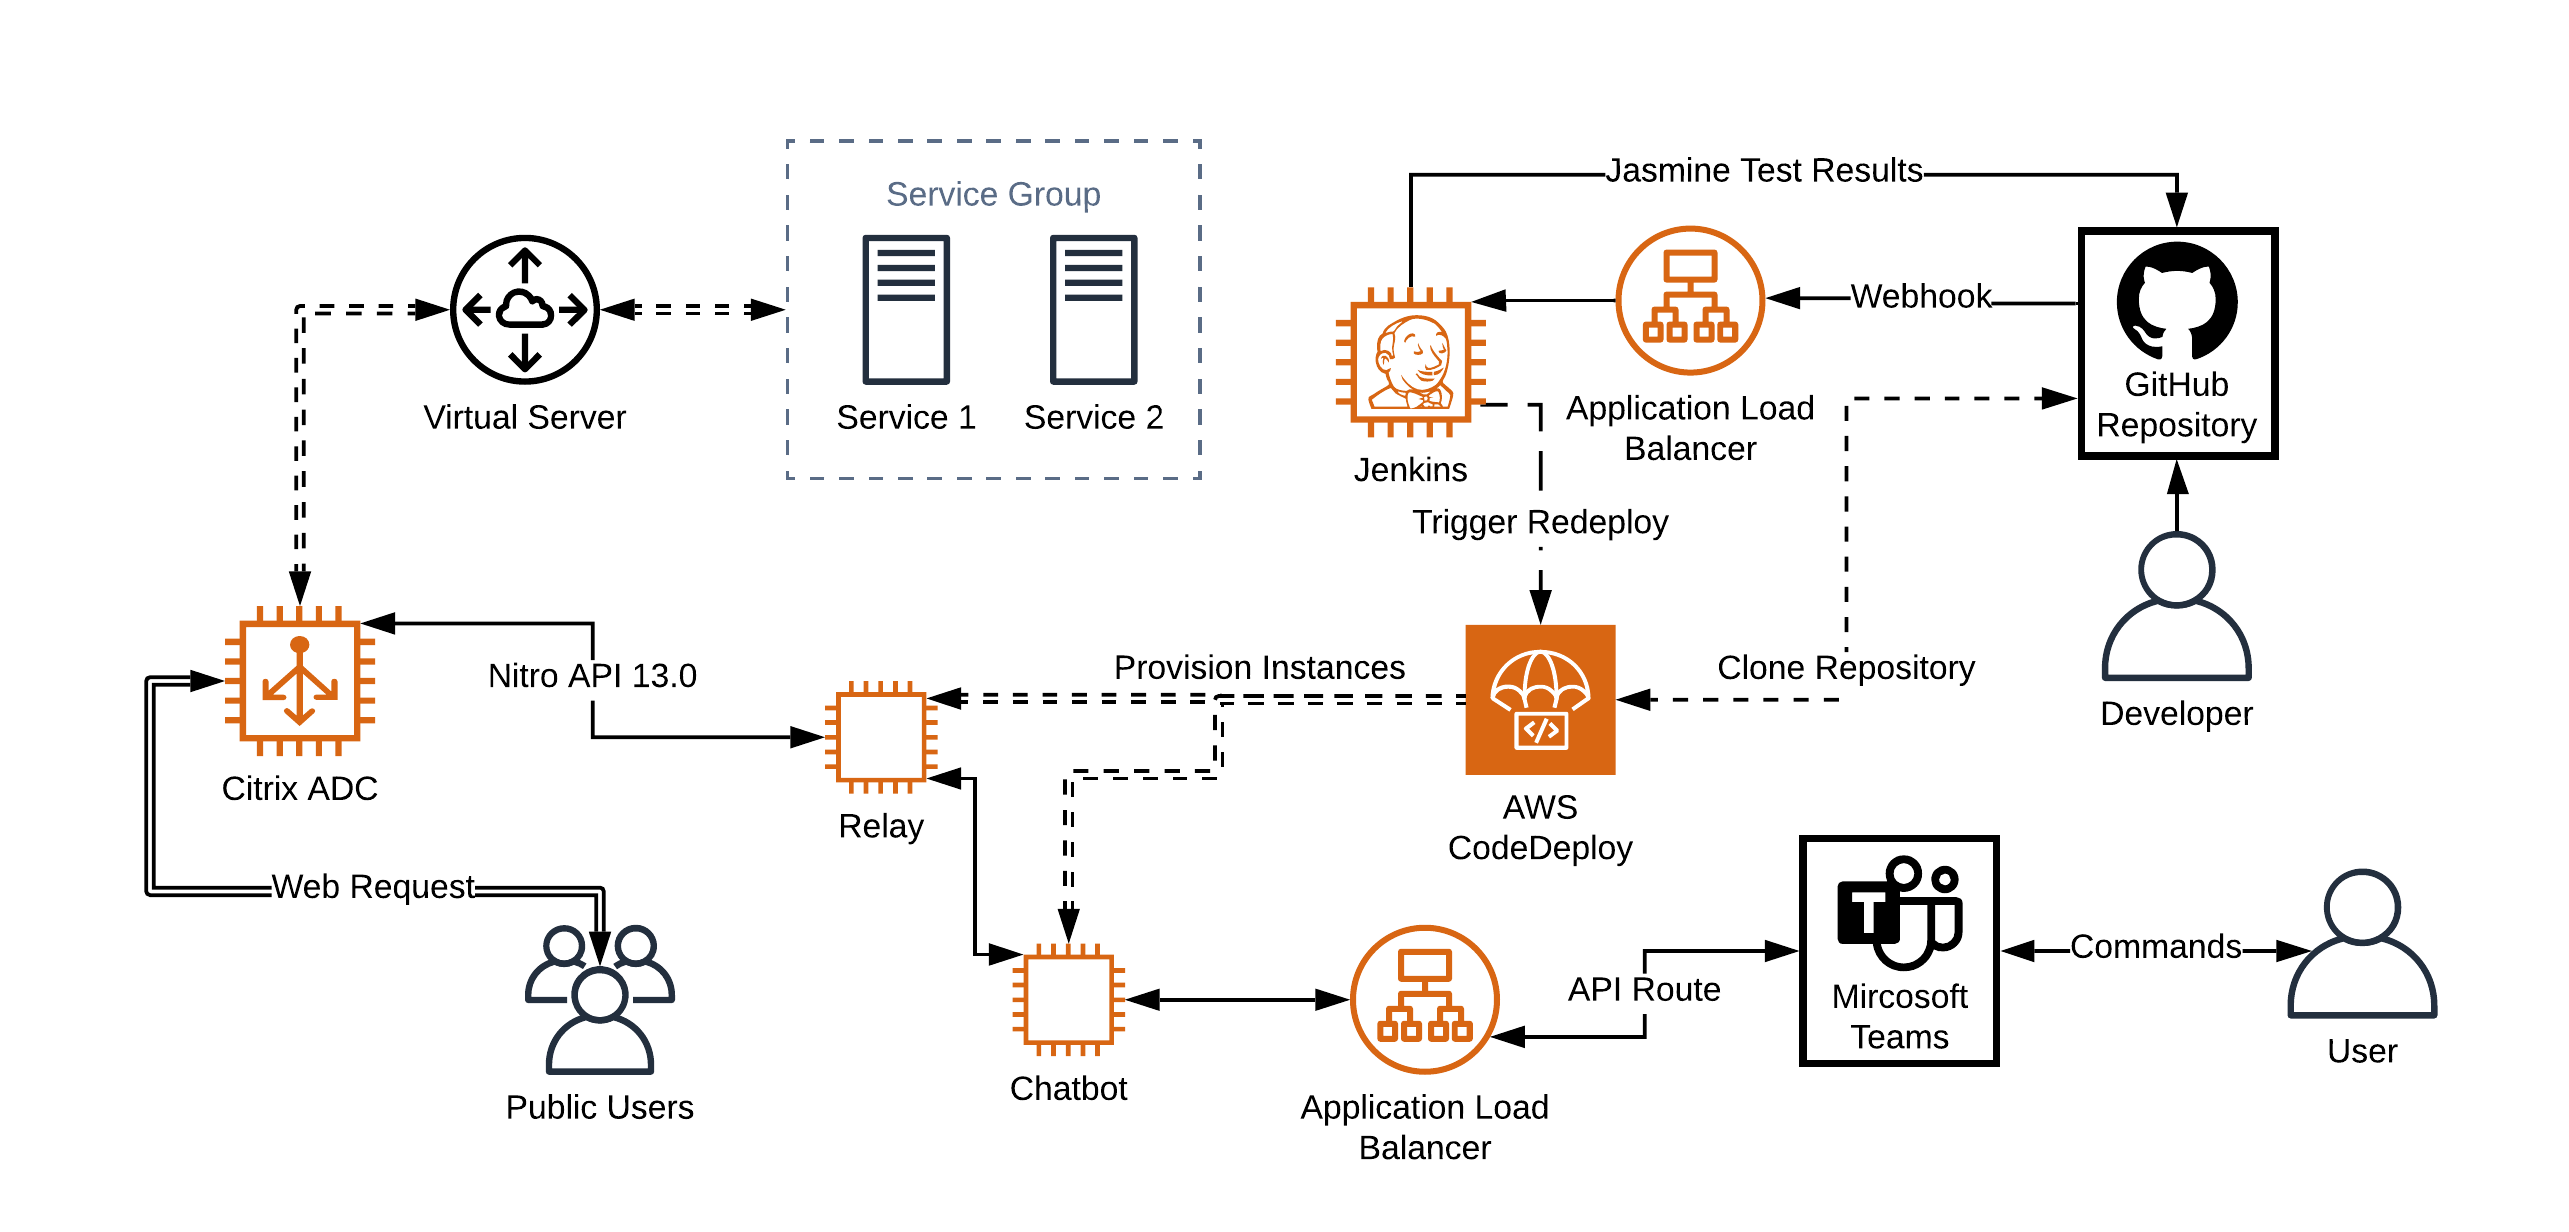
\includegraphics[height=8cm]{projectdiagram.png}
    \caption[Project Diagram]{Diagram showing the connectivity of different project components}
    \label{fig:Project Diagram}
\end{figure}
\subsection{Current State}
Currently our project is operational, missing only a couple key components to reach our final target.
Above (Fig. 1) you can see a graphical representation of our current implementation.
Any icon that is colored orange represents an instance or usage of an AWS service.

Currently, all the main code is written, and operation of the chatbot is demoed in our video.
The chatbot handles all user messages, giving correct errors for any inputs that don't match the required pattern.
This method for reading messages most closely emulates a command-line style, which we know our users are familiar with.

Additionally from the chatbot component, all interactions are logged in AWS CloudWatchLogs.
This allows for administrative auditing, tracking any configuration modification in the event of a future issue.

Next the relay is completely operational as well, parsing all messages (securely) sent from the chatbot, and performing the correct operations.
Each request from the Chatbot causes the relay to re-authenticate, and preform a sequence of requests (sometimes 5 or 6 individual requests) to complete the action.
When the relay completes the request it received, it's sends a response, formatted such that the chatbot can parse and print it in a reply to the user.

Even given the relatively low powered instances we are using for our project, the most complex of requests only takes a couple seconds to complete (well below the required metric of 60 seconds).

Of particular note, is the complexity of the program given the possible number of errors that may occur when dealing with 3 total servers for each request (in addition to communication through Microsoft's services and AWS for logging).
The entire project must account for errors at every stage, and be prepared to provide adequate feedback to the user.

For the deployment component of our assignment, we sent up an AWS Instance for Jenkins.
Jenkins is essential a build server, which, among many other things, can be used to automate tasks with projects such as ours.
We configured our instance of Jenkins to automatically pull code pushed to our GitHub repository, run our Jasmine tests, and report to results back to GitHub.
This is achieved using web hooks from GitHub, which can be configured to send updates about our repository to remote servers.

\subsection{Remaining Tasks}
There are a few tasks that are left to complete in the project.
First, the Chatbot does not yet operate within Microsoft Teams despite all the pre-requisites for doing so have been met.
We believe this to be a fairly simple issue involving the chatbot not being programmed to trigger on the correct event.

Regardless of this, an application manifest has been completed, and the Chatbot is visible within Teams (Fig. 2).
We know the chatbot receives messages, it just doesn't trigger the correct event yet.

\begin{figure}[h]
    \centering
    \captionsetup{format=hang,justification=raggedright,margin=2cm}
    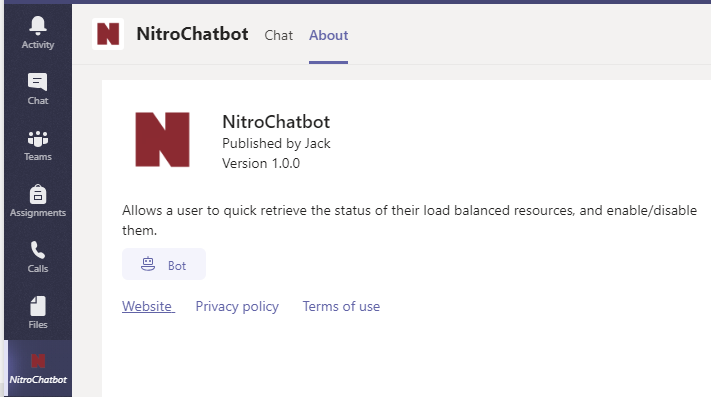
\includegraphics[height=5cm]{teamsapp.PNG}
    \caption[App within Teams]{Nitro Chatbot application About tab within Microsoft Teams}
    \label{fig:Teams App About Page}
\end{figure}

The next task is to usage of a database beyond a simple file.
Currently, the relay uses a locally stored CSV file to match pre-authenticated user IDs to NetScaler credentials.
While this current method works well, we believe that a better solution exists.
Originally, we thought we may leverage OSU's identity provider to replace an active database.
However actual implementation of federated logins, tunneled through so many servers, is tricky at best.

The next remaining task is creating meaningful test suites.
While the team wanted to tackle this task first, the actual organization of our code base was still in the air.
This made writing tests tricky, especially given that input for our chatbot is tunneled through BotKit, the Node.JS package we are using to provide access to Microsoft Teams.
Now that our code structure is more stable, we do have some ideas on how to more rigorously test parts of our code (especially error handling).

The final remaining task for our project is to complete the deployment portion of our CI/CD pipeline.
Currently, deployments and updates are done manually, which is inefficient and a bit annoying when testing Teams integration.
The plan is to have Jenkins's trigger AWS CodeDeploy redeployments for the Chatbot and Relay instance.

\section{Project Progress}
\subsection{Problems & Solutions}
%    describe any problems that have impeded your progress, with any solutions you have
We had a couple problems that had impeded our progress.
First we have problems establishing our development environment, as team members were using different operating systems on their development laptop.
To overcome this issue, a development Virtual Machine was created by one of the team members.
By creating a single VM pre-loaded with the needed software, team members were all able to work on the project unimpeded by system differences.

The next problem that we encountered was getting the proper version of the NetScaler software running remotely, so that were could query it from AWS.
Our requirements document specifies we use NITRO 12.0, which is compatible with the NetScaler 12.0 software.
Despite having access to an appliance with this version of NetScaler, it was difficult to find a way to host it remotely.

Eventually the team decided to instead run an up-to-date instance using Citrix ADC 13.0 (which includes NetScaler capability within it's software).
This version of software is available as a pre-build AMI (Amazon Machine Image) available for use within AWS instances.
The team found no notable difference between the 2 versions of Nitro for the applications purposes.
Regardless, the code is organized to allow for different URLs between Nitro Versions if one is found through our final testing.

\subsection{Interesting Implementations}
One particularly interesting solution (and piece of code) that I wanted to talk about is our solution to a problem mentions during our presentation.

At the time, we had no way to guarantee that the relay would only accept messages from the chatbot.
It was possible that a 3rd party could inject messages to our relay.
While this could be protected against in AWS using security groups, the final deployment would have these communications running across public internet.

After some thought we decided on a solution that is often used as dual-factor authentication.
The basic idea is that both parties have a shared secret key (a symmetrical key), and every 30 seconds that same key generates a different 6 digit code.
Without the symmetrical key, it's impossible to guess the next code.
For our project, we have the chatbot generate a code and add it along in it's request body (Fig. 3).

\begin{figure}[h]
    \centering
    \captionsetup{format=hang,justification=raggedright,margin=2cm}
    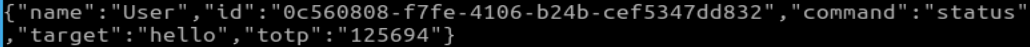
\includegraphics[height=.7cm]{totpobject.png}
    \caption[Communication JSON]{Each request to the relay contains a JSON with this format, including a TOTP Key.}
    \label{fig:Communication JSON}
\end{figure}

To generate the TOTP key, we used a pre-built module, which uses the approved RFC method for generating a TOTP (Time One Time Password).
However to validate the key required a working knowledge of the generation algorithm, and a small modification to the module.
Below (Fig. 4) you can see the code used for validating the key.
What's special about the validation method is that you need a built-in tolerance, checking previous and future keys, in case of a delayed message.
I'm particularly fond of the simple solution to what could have been a much larger problem.

\clearpage
\section{Appendices}
\subsection{TOTP Validation Code}
\begin{figure}[h]
    \centering
    \captionsetup{format=hang,justification=raggedright,margin=2cm}
    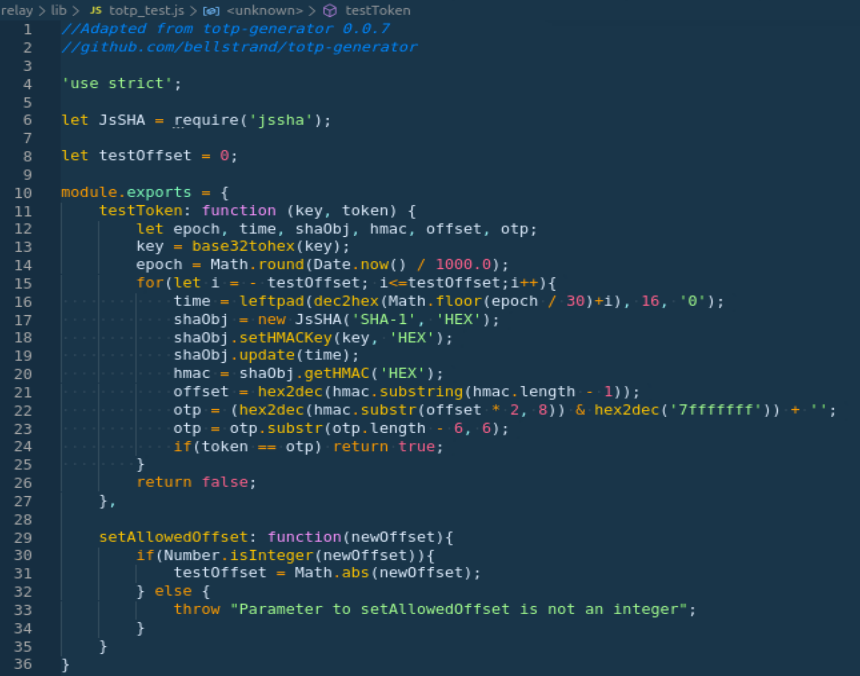
\includegraphics[height=9cm]{totp.png}
    \caption[TOTP Validation]{Node JS code showing a TOTP library modified for validation checking.}
    \label{fig:TOTP Validation}
\end{figure}

\subsection{Available User Commands}
\begin{figure}[h]
    \centering
    \captionsetup{format=hang,justification=raggedright,margin=2cm}
    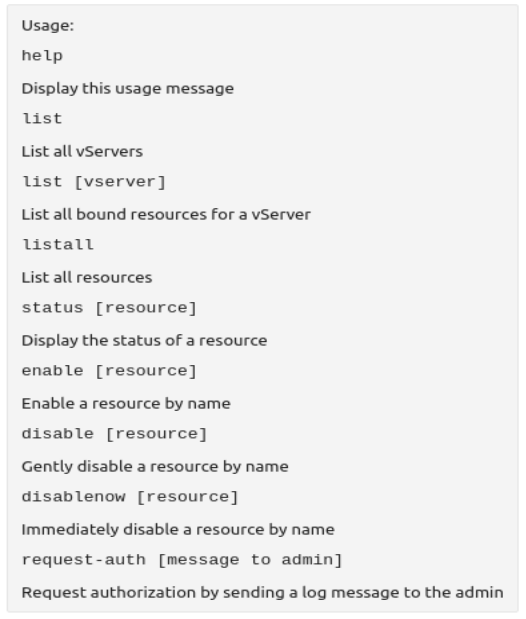
\includegraphics[height=8cm]{usercommands.png}
    \caption[User Commands]{Available user commands}
    \label{fig:Commands}
\end{figure}

%\clearpage
%\bibliographystyle{IEEEtran}
%\bibliography{dd}
\end{document}

%\subsection{Remaining Tasks}